\documentclass[times, utf8, seminar, numeric, tikz]{fer}
\usepackage{booktabs}
\usepackage{url}
\usepackage[final]{pdfpages}
\usepackage{amsmath}
\usepackage{blindtext}
\usepackage{enumitem}
\usepackage{listings}


\renewcommand{\lstlistingname}{Programski isječak}% Listing -> Algoritam
\renewcommand{\lstlistlistingname}{Popis programskih isječaka}% List of Listings -> Popis algoritama 


\definecolor{codegreen}{rgb}{0,0.6,0}
\definecolor{codegray}{rgb}{0.5,0.5,0.5}
\definecolor{codepurple}{rgb}{0.58,0,0.82}
\definecolor{backcolour}{rgb}{0.95,0.95,0.92}
\definecolor{keyword}{rgb}{0,0,0}

\lstdefinestyle{mystyle}{
	backgroundcolor=\color{backcolour},   
	commentstyle=\color{codegreen},
	keywordstyle=\bfseries\color{keyword},
	numberstyle=\tiny\color{codegray},
	stringstyle=\color{codepurple},
	basicstyle=\footnotesize,
	breakatwhitespace=false,         
	breaklines=true,                 
	captionpos=b,                    
	keepspaces=true,                 
	numbers=left,                    
	numbersep=5pt,                  
	showspaces=false,                
	showstringspaces=false,
	showtabs=false,                  
	tabsize=4,
	inputencoding=utf8,
	morekeywords={vrati, ako, za\_svaki, prekini\_petlju} 
}	
	
	


\lstset{style=mystyle,texcl=true}
% set font translations
%\lstset{inputencoding=utf8}
\lstset{extendedchars=true}
\lstset{
	literate=%
	{ć}{{\'c}}1
	{č}{{\v{c}}}1
	{đ}{{\dj{}}}1
	{š}{{\v{s}}}1
	{ž}{{\v{z}}}1
	{Ć}{{\'C}}1
	{Č}{{\v{C}}}1
	{Đ}{{\DJ{}}}1
	{Š}{{\v{S}}}1
	{Ž}{{\v{Z}}}1
}

\begin{document}
\pagenumbering{gobble}

% Ukljuci literaturu u seminar
\nocite{*}

% TODO: Navedite naslov rada.
\title{Algoritam Minimaks i primjena na igru "4 u nizu"}

% TODO: Navedite vaše ime i prezime.
\author{Kristijan Vulinović}

% TODO: Navedite ime i prezime voditelja.
\voditelj{Doc. dr. sc. Marko Čupić}

	\maketitle


\tableofcontents

\chapter{Uvod}

Umjetna inteligencija je u današnje vrijeme jedna od najbrže rastućih grana računarstva. Primjenjuje se u raznim područjima poput zdravstva, ekonomije, proizvodne industrije, čak i avijacije. Osim navedenoga, umjetna inteligencija se intenzivno koristi i u brojnim računalnim igrama.\\

U daljnjem tekstu ćemo posvetiti pozornost specifičnoj skupini igara; igrama ukupne sume nula, koje su detaljnije opisane u \cite{5205101}. U njima sudjeluje više igrača koji međusobno imaju dijametralno suprotne interese. Na primjeru igre za dva igrača, to bi značilo da ako jedan pobijedi, drugi je nužno izgubio i obrnuto. I dalje je moguć scenarij neriješenog ishoda, no taj je rezultat lošiji od pobjede, ali bolji od gubitka, čime ukupna "suma" rezultata ostaje konstantna. Bitno je primijetiti kako nije dozvoljena situacija u kojoj oba igrača pobjeđuju, niti situacija u kojoj oba gube. Posebna kategorija takvih igara su igre potpune informacije u kojima svi igrači imaju uvid u sve što se događa u igri.\\

Najpoznatija, a ujedno i vrlo jednostavna igra ovog svojstva je \textit{križić-kružić}. U njemu sudjeluju dva igrača koji naizmjence u polje kakvo je prikazano na slici \ref{fig:tttPolje} upisuju znakove \textit{$"X"$ }, odnosno \textit{$"O"$ }. Pobjednik je onaj koji prvi uspije upisati tri znaka u nizu; vodoravno, okomito ili dijagonalno. Ako niti jedan od igrača to ne uspije, a cijelo je polje popunjeno, igra završava neriješenim rezultatom. Dodatno svojstvo ove igre je da uvijek završava neriješenim rezultatom ako oba igrača igraju optimalno.\\

\begin{figure}[h] 
	\centering
	\includegraphics[width=0.185\linewidth]{Samples/emptyField.pdf}
	\caption{Polje za križić-kružić}
	\label{fig:tttPolje}
\end{figure}  

\chapter{Algoritam Minimaks}
\section{Način rada algoritma}
Prilikom analiziranja igre, cilj je pronaći potez koji će garantirati pobjedu ako je to moguće. Ako takav potez nije moguće pronaći, cilj je pronaći potez koji će rezultirati najboljim mogućim ishodom. Kako bi se to postiglo, pretpostavlja se kako protivnik igra optimalno. Tu pretpostavku se smije učiniti zahvaljujući tome što ona predstavlja najgori mogući scenarij za trenutnog igrača. Ako naš protivnik ne igra optimalno, igrač se i dalje osigurao da njegov potez vodi najboljem mogućem rezultatu.\\

Najbolji mogući potez odabire se tako da se isprobaju svi trenutno mogući potezi. Ako neki od njih odmah dovodi do stanja u kojemu je igra gotova, računaju se bodovi koji se ostvaruju i nastavlja se pretraga s ostalim potezima. Ako potez nije završni, analiza će se nastaviti tako da se gleda što protivnik može odigrati za svaki od mogućih poteza. Njegovi potezi se također gledaju tako da se provjeravaju sve mogućnosti, no ovaj puta ako on može odigrati potez takav da je odmah pobijedio, taj potez se smatra lošim za trenutnog igrača. Ostali potezi ponovno se analiziraju tako da se isprobaju sve mogućnosti koje postoje i postupak se ponavlja sve dok se ne dobije ishod svakog mogućeg poteza. Jednom kad se to napravi, trivijalno je za odabrati najbolji potez zahvaljujući prikupljenim ishodima.\\

\begin{figure}[h]
	\centering
	\includegraphics[width=0.7\linewidth]{Samples/tttExample.pdf}
	\caption{Primjer grafa stanja za jednu situaciju}
	\label{fig:minMaxExample}
\end{figure}  

Primjer takve analize ta igru "križić-kružić" prikazan je na slici \ref{fig:minMaxExample}. Radi lakšeg razumijevanja, dobitna stanja (gledano iz perspektive igrača s oznakom $"X"$ ) označena su znakom "+", gubitna znakom "-", a stanja u kojima je rezultat neriješen označena su znakom "=". Ako je poznato da je na potezu igrač s oznakom $"X"$, očevidno je kako mu na raspolaganju stoje tri različita poteza. Jedan od njih rezultira trenutnim dobitkom, na temelju čega je moguće odmah zaključiti da taj potez treba odigrati.\footnote{U općenitom slučaju ovo ne mora biti istinito. Općenita igra može imati više različitih pobjedničkih stanja, poput nekog koje donosi 4 boda pobjedniku i 1 bod gubitniku, i nekog drugog koje donosi 5 bodova pobjedniku i 0 bodova gubitniku. Za takvu igru također vrijedi da je igra konstantne sume. U tom slučaju nije dovoljno zadovoljiti se prvim pronađenim dobitkom, već treba pronaći dobitak koji će donjeti najveći broj bodova.} No ukoliko treba odrediti ishode ostalih poteza potrebno je nastaviti s daljnjom pretragom mogućnosti. Potez koji je prikazan u sredini drugog retka na slici \ref{fig:minMaxExample} ne vodi do trenutnog rezultata. Analiza se nastavlja provjerom poteza protivnika. Vidi se kako on ima dvije mogućnosti; jednu u kojoj se igra dalje nastavlja te početnom igraču ostaje samo jedno slobodno polje koje završava neriješenim rezultatom, i jednu u kojoj je on pobijedio. Situacija u kojoj je protivnik pobijedio tretira se kao gubitak za trenutnog igrača, što se može učiniti zahvaljujući činjenici da je ovo igra konstantne sume. Poznavanjem svih mogućih ishoda nakon što se odigra ovaj potez, zaključuje se kako će igrač igranjem tog poteza izgubiti. Zadnji preostali potez je onaj prikazan na desnoj strani drugog retka. U novonastaloj situaciji, protivnik ponovno može odigrati dva različita poteza; nakon jednoga preostaje samo jedan potez nakon kojega je igra završila neriješeno, nakon drugoga preostaje samo jedan potez nakon kojega je trenutni igrač pobjedio. Uz navedenu pretpostavku da protivnik igra optimalno, zna se kako on neće odigrati potez nakon kojega trenutni igrač pobjeđuje, već potez nakon kojega igra završava neriješeno. Generalno, može se reći kako će igranje tog poteza završiti neriješenim rezultatom. Sada kad su određeni ishodi svih mogućih poteza, vidljivo je kako je jedini potez kojeg se smije odigrati onaj koji je prikazan lijevo u drugom retku slike \ref{fig:minMaxExample}, jer jedino taj potez vodi do sigurne pobjede.

\section{Implementacija}
Implementacija algoritma podijeljena je u dva razreda; pomoćni razred koji nudi metode specifične za određenu igru, i razred koji implementira metode algoritma. Na taj način nastaje generaliziran program koji se uz modifikaciju jednog razreda može koristiti za bilo koju drugu igru.\\

Za potrebe analiziranja trenutnog stanja igre potrebno je implementirati pomoćni razred koji nudi metode prikazane u nastavku.
\renewcommand{\labelitemi}{\textbullet }
\begin{itemize}
	\item \ttfamily mogućiPotezi(stanje, igrač) - \rmfamily za dano stanje igre vraća listu poteza koje navedeni igrač može odigrati
	\item \ttfamily odigraj(stanje, igrač, potez) - \rmfamily za dano stanje igre i potez koji treba odigrati vraća novo stanje koje prikazuje igru nakon što se odigra željeni potez
	\item \ttfamily provjeriKraj(stanje) - \rmfamily za dano stanje igre provjerava je li trenutno stanje kraj igre
	\item \ttfamily odrediBodove(stanje, igrač) - \rmfamily za dano stanje igre i trenutnog igrača određuje bodove koje je igrač osvojio. Metoda može biti korištena isključivo za stanja za koja bi metoda \ttfamily provjeriKraj(stanje) - \rmfamily vratila istinitu vrijednost.
	\item \ttfamily sljedećiIgrač(igrač) - \rmfamily za danog igrača vraća igrača koji je sljedeći na potezu
\end{itemize}
Sam algoritam implementiran je u zasebnom razredu, u kojemu je definirana jedna javna metoda koja kao argument prima trenutno stanje igre, a kao rezultat vraća potez koji treba odigrati.\\

\begin{minipage}{\textwidth}
	\lstinputlisting[caption = {Pseudokod metode minimax},label={fig:codeMinimax}]{Codes/minimax.txt}
\end{minipage}


Pseudokod opisane metode prikazan je u programskom isječku \ref{fig:codeMinimax}. Program radi tako da uz pomoć prethodno navedenog pomoćnog razreda dohvati sve moguće poteze u trenutnom stanju igre. Nakon toga se za svaki potez određuje vrijednost bodova koje će igrač skupiti igranjem tog poteza. Potom se određuje potez s najvećim brojem ostvarenih bodova te se taj potez vraća kao rezultat funkcije. \\

Broj bodova koje je moguće ostvariti igranjem pojedinog poteza određuje se pozivanjem privatne metode \ttfamily maxVrijednost\rmfamily, čiji je pseudokod prikazan u programskom isječku \ref{fig:codeMaxVal}. Navedena metoda prvo provjerava je li trenutno stanje kraj igre. Ako je, vraća broj bodova koje je igrač osvojio. U suprotnome metoda će provjeriti sve ostale poteze te odabrati onaj potez koji protivniku nudi najmanje moguće bodova. To će se dalje rekurzivno računati pozivanjem metode \ttfamily minVrijednost\rmfamily,\space čiji je pseudokod prikazan u programskom isječku \ref{fig:codeMaxVal}.\\

U navedenim isječcima se primjećuje sličnost dviju metoda, što proizlazi iz načina rada algoritma. Metoda \ttfamily maxVrijednost\rmfamily\space provjerava moguće poteze koje trenutni igrač može odigrati, zbog čega se odlučuje za potez s maksimalnim rezultatom. Za razliku od nje, metoda \ttfamily minVrijednost\rmfamily\space računa sve daljnje poteze protivnika, te je trenutnom igraču optimalno uzeti potez koji će igru dovesti u stanje u kojemu protivnik ima najmanji mogući rezultat.\\

\begin{minipage}{\textwidth}
	\lstinputlisting[caption = {Pseudokod metode maxVrijednost},label={fig:codeMaxVal}]{Codes/maxVrijednost.txt}
\end{minipage}

\begin{minipage}{\textwidth}
	\lstinputlisting[caption = {Pseudokod metode minVrijednost},label={fig:codeMinVal}]{Codes/minVrijednost.txt}
\end{minipage}

\section{Složenost}
Algoritam Minimaks koristi rekurzivno pretraživanje u dubinu za analizu stanja igre. Ako najveću dubinu stabla stanja označimo sa $m$, a broj poteza u svakom stanju sa $b$. Vremenska složenost pretrage je tada $O(b^m)$. Prostorna složenost je $O(bm)$ za algoritam koji generira sva stanja odjednom, odnosno $O(m)$ ako generira samo jedno stanje \cite{s.russellp.norvig2009}.\\

Složenost algoritma je prevelika za većinu igara, zbog čega nije praktičan za uporabu. Kako bi se to riješilo, uvodi se novi argument, najveća dozvoljena dubina pretrage. Rekurzija se poziva sve dok ne dođe do definirane najveće dubine, kada se prekida daljnje pretraživanje. Tada se stanje procjenjuje korištenjem heuristike. Takav pristup neće rezultirati nužno optimalnim potezom, ali se vrijeme izvođenja smanjuje na razinu koja je prihvatljiva, detaljnije objašnjenje moguće je pronaći u \cite{page1}. Pseudokod metode \ttfamily maxValue \rmfamily tada izgleda kao u programskom isječku \ref{fig:codeMaxDepth}. \\

\begin{minipage}{\textwidth}
	\lstinputlisting[caption = {Pseudokod metode maxVrijednost s ograničenom dubinom rekurzivnog spusta},label={fig:codeMaxDepth}]{Codes/maxDepth.txt}
\end{minipage}


Navedenim primjerom se i dalje održava odvajanje logike povezane uz igru i logike povezane s algoritmom. Osim promjena prikazanih u pseudokodu, potrebno je implementirati i metodu \ttfamily odrediBodoveHeuristički\rmfamily,\space koja je specifična za određenu igru te se nalazi u pomoćnom razredu.

\chapter{Alfa-beta podrezivanje}
\section{Način rada algoritma}
Problem algoritma Minimaks je u tome što nije dovoljno brz da bi bio primjenjiv u većini igara. Primjenom tog algoritma nije moguće je izbjeći eksponencijalnu složenost, ali je ipak moguće djelomično smanjiti eksponent. Osnovna ideja temelji se na tome da je u određenim slučajevima moguće odrediti optimalan potez bez da se provjere sva moguća stanja, što je opisano u \cite{s.russellp.norvig2009}.\\

\begin{figure}[h]
	\centering
	\includegraphics[width=0.7\linewidth]{Images/minimaxExample}
	\caption{Potpuni graf stanja \cite{s.russellp.norvig2009}}
	\label{fig:minimaxExample}
\end{figure}

Na slici \ref{fig:minimaxExample} prikazan je graf stanja neke igre. Trenutno stanje je stanje označeno slovom \textit{A}, a korištenjem algoritma Minimaks dobivene su vrijednosti prikazane uz svaki od čvorova. Stanje \textit{B} donosi najveći mogući broj bodova te je optimalno odigrati potez \textit{a1} kako bi se došlo u to stanje.\\

\begin{figure}[h]
	\centering
	\includegraphics[width=1.0\linewidth]{Images/alphaBetaIspravak}
	\caption{Postupna pretraga korištenjem podrezivanja alfa-beta\cite{s.russellp.norvig2009}}
	\label{fig:alphaBetaExample}
\end{figure}

Jednak rezultat moguće je dobiti i na drugi način, kao što je prikazano na slici \ref{fig:alphaBetaExample}. Analiza započinje korištenjem klasičnog algoritma Minimaks, ali uz jedan dodatak. U svakom stanju dodatno se pamti najveća i najmanja moguća vrijednost za koje je utvrđeno da mogu biti rezultat algoritma. Ti parametri se uobičajeno nazivaju alfa (najmanja moguća vrijednost) i beta (najveća moguća vrijednost), po čemu je algoritam dobio ime. Korištenjem tih parametara cijelo vrijeme se prati interval unutar kojega se rješenje može nalaziti, a u slučaju da je dobiven nemoguć interval, zaključuje se kako optimalno rješenje nije u trenutnome podstablu. Na početku se rješenje nalazi unutar intervala $[+\infty, -\infty]$, što se uzima za početne vrijednosti parametara alfa i beta. U (a) dijelu slike \ref{fig:alphaBetaExample} provjerava se krajnje lijevo podstablo. Algoritam treba odrediti maksimalnu vrijednost prve razine, odnosno minimalnu vrijednost druge razine. Prva vrijednost koja je izračunata je 3, iz čega se zaključuje kako rezultat tog podstabla sigurno neće biti veći od 3, budući da se određuje minimalna vrijednost. Parametar beta postavlja se na 3 iz čega se zna da je rješenje tog podstabla unutar intervala $[-\infty, 3]$. U (b) dijelu se nastavlja računanje ostalih stanja te se provjerava stanje čija je vrijednost 12. To je veće od trenutnog minimuma te ništa ne treba mijenjati. Sljedeće stanje koje se provjerava u (c) dijelu slike ima vrijednost 8. Vrijednost stanja \textit{B} sada je u potpunosti izračunata i iznosi 3. Daljnja pretraga nastavlja se u stanju \textit{C}. Prethodno je izračunato kako postoji stanje čiji je rezultat 3. Poznavajući taj rezultat, sigurno je da se nikada neće odabrati manji rezultat, odnosno da će svi rezultati biti u intervalu $[3, +\infty]$. Prvo sljedeće pregledano stanje vraća vrijednost 2. Na toj razini odabire se najmanji rezultat, iz čega se zaključuje da se nikada neće odabrati rezultat veći od 2. Interval u kojemu se očekuje rezultat je $[3, 2]$, što nije moguće. Daljnja pretraga stanja \textit{C} se prekida jer bez obzira na ostale vrijednosti, ovo stanje sigurno nije optimalno. U (e) dijelu slike prikazana je pretraga za stanje \textit{D}, čiji rezultat može biti unutar intervala $[3, +\infty]$. U lijevom dijelu podstabla vrijednost je 14, zbog čega se interval rješenja sužava na $[3, 14]$. Sljedeći rezultat je 5, zbog čega se parametar beta smanjuje na 5 te rezultat može biti unutar intervala $[3, 5]$ Zadnji preostali rezultat ovog podstabla je 2, zbog čega se interval u kojemu rješenje može biti sužava na $[3, 2]$. Ovaj interval također nije moguć te se daljnja pretraga prekida. Nakon ove analize odabire se stanje \textit{B} kao optimalno, odnosno igra se potez koji dovodi do tog stanja, što je isto rezultatu koji je odredio običan algoritam Minimaks. Zahvaljujući parametrima alfa i beta koji su određivali granice intervala u kojemu se rješenje može nalaziti, moguće je za prikazani primjer odrediti točan rezultat bez provjere 2 stanja, odnosno svih stanja koja slijede nakon njih.

\section{Redoslijed poteza}
Opisani algoritam uvijek će odrediti ispravan rezultat, ali vrijeme izvođenja može se značajno razlikovati ovisno o redoslijedu obilaska poteza koji se mogu odigrati. U primjeru na slici \ref{fig:alphaBetaExample} prikazano je kako određena podstabla nije bilo potrebno proučavati. U tom primjeru ja za podstablo stanja \textit{C} trebalo proći kroz sva podstabla, a tek na zadnjemu se dogodio slučaj u kojemu je alfa parametar veći od beta parametra, zbog čega se ta pretraga prekinula. Kada bi se postiglo da algoritam za stanje \textit{C} prvo provjerava krajnje desno podstablo, odmah nakon prve izračunate vrijednosti bilo bi moguće prekinuti daljnju analizu. Tako bi se izbjeglo računanje preostala dva stanja u podstablu te bi za ovaj konkretan primjer izračun bio brži.\\

Kada bi bilo moguće odrediti funkciju koja bi moguće poteze vratila u takvom redoslijedu da je prvi potez ujedno i optimalan potez, složenost podrezivanja alfa-beta bila bi $O(b^{m/2})$, za razliku od složenosti $O(b^m)$ kod algoritma Minimaks. Na taj bi se način najveća dubina pretrage mogla udvostručiti u odnosu na klasični algoritam Minimaks, a vrijeme pretrage se pritom ne bi promijenilo. Prethodno opisanu funkciju nije moguće ostvariti (kada bi to bilo moguće, ne bi bilo potrebno provoditi ovaj algoritam već bi se samo slijedili potezi u redoslijedu koji vraća ta funkcija). Unatoč tome, različitim metodama moguće je dobiti bolju složenost algoritma. Ako se mogući potezi obilaze u nasumičnom redoslijedu, složenost će iznositi $O(b^{3m/4})$. Korištenjem heuristike moguće je postići složenost koja bi bila još bliža minimalnoj mogućoj \cite{s.russellp.norvig2009}.

\section{Implementacija}

\begin{minipage}{\textwidth}
	\lstinputlisting[caption = {Pseudokod metode za poziv podrezivanja alfa-beta},label={fig:codeAlfaBeta}]{Codes/alfaBeta.txt}
\end{minipage}


U programskom isječku \ref{fig:codeAlfaBeta} prikazan je pseudokod implementacije podrezivanja alfa-beta. Metoda prima jednake argumente kao i običan algoritam Minimaks, te dodatno postavlja parametre alfa i beta na $-\infty$, odnosno $+\infty$. U pozivu metode \ttfamily maxVrijednost \rmfamily prosljeđuju se argumenti alfa i beta. Nakon što se izračunaju bodovi za određeni potez, provjerava se jesu li ti bodovi bolji od prethodno pronađenih najboljih bodova. Nakon toga treba provjeriti jesu li ti bodovi veći od parametra alfa. Ako jesu, zaključuje se kako sigurno neće biti odabran potez koji donosi manje bodova od trenutno izračunatih te se alfa parametar postavlja na novo izračunatu vrijednost. Potrebno je još provjeriti i je li trenutna vrijednost parametra alfa veća od vrijednosti parametra beta, što bi značilo da ne postoji rješenje u trenutno zadanom intervalu. Ako je taj uvjet ispunjen potrebno je prekinuti daljnju pretragu i vratiti do sada najbolje izračunati potez.\\

Pseudokod implementacije metode \ttfamily minVrijednost \rmfamily prikazana je u programskom isječku \ref{fig:codeAlfaBetaMin}. Pseudokod je vrlo sličan onome u programskom isječku \ref{fig:codeMinVal}, uz dodatak dvaju argumenata, alfa i beta. Slično isječku \ref{fig:codeAlfaBeta}, provjerava se jesu li trenutno najbolji bodovi manji od parametra beta. Ako jesu, parametar beta poprima vrijednost trenutno najboljih bodova. To neće utjecati na rezultat jer ova metoda bira najmanju vrijednost i sigurno neće odabrati niti jednu vrijednost veću od trenutne, zbog čega se interval u kojemu se nalazi rješenje može smanjiti. Ako je parametar alfa veći od parametra beta, interval ne sadrži niti jednu vrijednost u sebi te se daljnja pretraga prekida.

\begin{minipage}{\textwidth}
	\lstinputlisting[caption = {Pseudokod metode minVrijednost kod podrezivanja alfa-beta},label={fig:codeAlfaBetaMin}]{Codes/minAlfaBeta.txt}
\end{minipage}


Pseudokod metode \ttfamily maxVrijednost \rmfamily vrlo je sličan onome iz programskog isječka \ref{fig:codeMaxVal}, uz preinake koje su prikazane u isječcima \ref{fig:codeAlfaBeta} i \ref{fig:codeAlfaBetaMin}, zbog čega se neće zasebno prikazivati.

\chapter{Primjena u igri 4 u nizu}
\section{Pravila igre}
Igra "4 u nizu" igra se na ploči visine 6, a širine 7 polja, kao što je prikazano na slici \ref{fig:4inRow_board}. U igri sudjeluju dva igrača koji naizmjence ubacuju žetone svoje boje. Žeton je moguće postaviti u bilo koji nepopunjeni stupac te će on pasti na dno tog stupca, odnosno na posljednje postavljeni žeton u tom stupcu. Cilj igre je napraviti niz od 4 uzastopna žetona u svojoj boji. Žetoni se mogu nalaziti uzastopno vodoravno, okomito ili dijagonalno. Ova igra je također primjer igre konačne sume, a za razliku od igre "Križić-kružić", prvi igrač će uvijek pobijediti ako igra optimalno.\\

\begin{figure}[h]
	\centering
	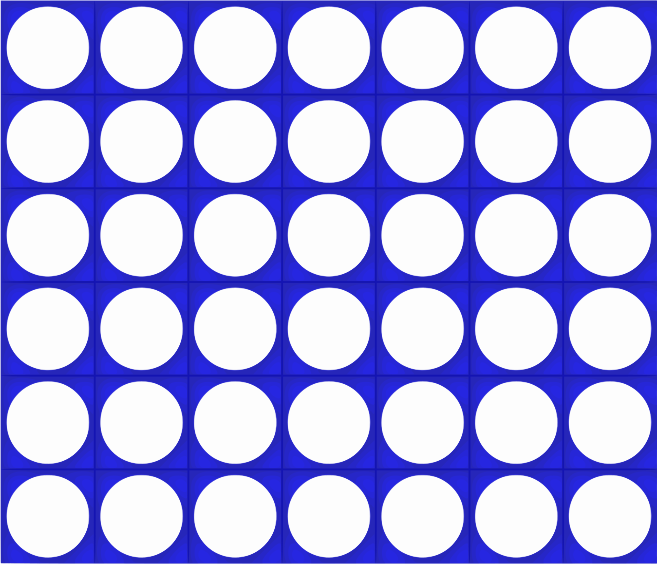
\includegraphics[width=0.75\linewidth]{Images/4inRow_board}
	\caption{Polje za igru 4 u nizu}
	\label{fig:4inRow_board}
\end{figure}

\section{Pomoćni razred}
Za potrebe ove igre razvijen je pomoćni razred, kao što je opisano u implementaciji algoritma Minimaks. Odigrani potezi pohranjuju se u listu brojeva, gdje svaki broj predstavlja stupac u kojega je određeni igrač ubacio žeton. Brojevi s parnim indeksima predstavljaju poteze prvoga, dok potezi s neparnim indeksima predstavljaju poteze drugog igrača. Takav zapis je praktičan za dodavanje novih poteza, ali ne omogućava jednostavan način provjere pobjednika u određenoj situaciji. Kao rješenje tog problema koristi se metoda koja listu poteza pretvara u matricu. Svako polje matrice predstavlja jedno polje ploče za igru, te poprima vrijednost koja označava je li to polje prazno ili se u njemu nalazi jedan od dva moguća žetona. Tako dobivenu matricu moguće je iscrpnom pretragom (engl. \textit{brute force}) provjeriti i ustanoviti je li igra završena te na isti način odrediti pobjednika ako postoji.

\section{Primjena algoritma Minimaks}
Algoritam Minimaks implementiran je kao što je opisano u programskom isječku \ref{fig:codeMaxDepth}. Dobiveni program dovoljno je efikasan za pobijediti prosječnog ljudskog protivnika, ali postoji još mnogo stvari koje se mogu unaprijediti. Trenutno opisani program provodi pretragu do dubine 6, kada prekida pretragu, a poziciju vrednuje kao izjednačenu.

\begin{figure}[h]
	\centering
	\includegraphics[width=0.75\linewidth]{Graphs/minimax}
	\caption{Vrijeme izvođenja algoritma Minimaks}
	\label{fig:grafMinimaks}
\end{figure}

Na slici \ref{fig:grafMinimaks} prikazano je vrijeme koje je programu potrebno za odrediti sljedeći potez, za dubinu pretrage 6.\footnote{Mjerenje je provedeno nad 250 odigranih igara. Pojedinačni rezultat za svaki potez po redu dobiven je kao aritmetička sredina svih izmjerenih vremena za taj potez. Sva mjerenja su provedena na računalu s Intel\textsuperscript{\textregistered} Core\texttrademark \space i7-4702MQ procesorom s radnim taktom u rasponu od $2,2$GHz do $3,2$GHz. Svi testirani programi napisani su korištenjem programskog jezika Java, verzija 1.8.077} Na grafu je vidljivo kako vrijeme potrebno za izračun određenog poteza nije jednako za svaki potez. Za izračun prvog poteza potrebno je prosječno 1,4 sekunde. Ta vrijednost raste do 1,8 sekundi za 9. potez, nakon čega vrijeme potrebno za izračun pada prema nuli. Ovakvo ponašanje programa je očekivano, a može se objasniti brojem različitih stanja igre. Na početku igre moguće je uvijek odigrati 7 različitih poteza, što uzrokuje veliki faktor grananja rekurzije. Nakon odigranih 8 poteza moguće je očekivati pobjedu jednog igrača, što kao posljedicu ima stanja koja su završna. Program prilikom pretraživanja svih stanja može naići na takvo stanje na dubini manjoj od 6, nakon čega neće morati provjeravati veće dubine tog podstabla.

\section{Optimizacija primjenom podrezivanja alfa-beta}
Prva mogućnost optimizacije je primjena podrezivanja alfa-beta, kao što je prethodno opisano. 

\begin{figure}[h]
	\centering
	\includegraphics[width=0.75\linewidth]{Graphs/alphabeta}
	\caption{Vrijeme izvođenja korištenjem podrezivanja alfa-beta}
	\label{fig:grafAlfaBeta}
\end{figure}

Graf na slici \ref{fig:grafAlfaBeta} prikazuje vrijeme koje je programu koji koristi podrezivanje alfa-beta potrebno za odrediti sljedeći potez. Svi uvjeti testiranja bili su jednaki onima iz prethodnog primjera. Kao i očekivano, graf ima sličan oblik onome na slici \ref{fig:grafMinimaks}, ali se primjećuje kako je izvođenje višestruko brže. Umjesto prethodnih 1,4 sekunde u najgorem slučaju, programu je trebalo nešto manje od 0,13 sekunde. Ubrzanje iznosi preko 10 puta, u prosječnom slučaju. Dodatno ubrzanje može se postići i drugačijim odabirom poteza. Osim prethodno testiranog programa, u kojemu se potezi provjeravaju redom od prvog do zadnjeg stupca, testirana su još dva drugačija pristupa; jedan u kojemu se potezi provjeravaju u nasumičnom redoslijedu, drugi u kojemu se potezi provjeravaju počevši od sredine. 

\begin{figure}[h]
	\centering
	\includegraphics[width=0.75\linewidth]{Graphs/podrezivanja}
	\caption{Vrijeme izvođenja korištenjem podrezivanja alfa-beta}
	\label{fig:grafPodrezivanja}
\end{figure}

Na slici \ref{fig:grafPodrezivanja} prikazana su vremena izvođenja svih triju implementacija. Pokazalo se kako nasumičan odabir poteza prilikom daljnje pretrage ima slično vrijeme izvođenja poput onoga kada se prvo provjerava središnji stupac. Iz grafa se također vidi kako predložene dvije metode u prosjeku imaju kraće vrijeme izvođenja od početnog programa. Umjesto 130 milisekundi koje je početni program trebao u prosječno najgorem slučaju, testirani programi izvode se u malo više od 100 milisekundi, što predstavlja dodatno ubrzanje od $25\%$, odnosno oko 14 puta u odnosu na početni algoritam.

\section{Izrada heuristike}
Za potrebe ovog rada razvijena su tri različita rješenja pomoću kojih se stanje u igri vrednuje nakon postizanja najveće dozvoljene dubine pretrage. Prvo je da sva takva stanja ocjenjuje neutralnim rezultatom. To predstavlja rad programa koji radi bez korištenja ikakve heurističke metode. Drugo rješenje svakom stanju dodjeljuje nasumične bodove. Time se postiže da ako nije moguće doći do pobjede unutar sljedećih nekoliko poteza koliko je određenom dubinom pretrage, odabiremo nasumični potez od onih koji neće rezultirati gubitkom. Treće rješenje je heuristička metoda koja pokušava svakom stanju dodijeliti određen broj bodova, ovisno o tome koji igrač ima veću vjerojatnost za pobjedu. Bodovi se dodjeljuju na način da se prebroje sva pojavljivanja 2 uzastopna žetona jednog igrača u nizu. Taj broj se množi faktorom bodova koji je predviđen za tu pojavu, a tako dobiveni umnožak pridodaje se ukupnim bodovima tog stanja. Isto to se radi i za protivnika, uz razliku što se njegovi bodovi oduzimaju od ukupnih bodova. Isto to se radi i za nizove od 3 uzastopna žetona, što se množi faktorom predviđenim za taj slučaj. Dodatno, ukoliko postoji situacija u kojoj igrač ima 2 uzastopna žetona, nakon kojih dolazi jedno prazno polje, a nakon toga još jedan žeton tog igrača, ta se situacija također tretira kao 3 žetona u nizu. Analogno tome, 2 žetona između kojih se nalazi jedno prazno polje tretiraju se kao 2 uzastopna žetona.\\

Navedene faktore potrebno je odrediti, a ovisno o njihovim vrijednostima moguće je dobiti bolju ili lošiju procjenu situacije. Početno razmišljanje temelji se na tome da je igraču poželjno imati čim više pozicija u kojima ima dva uzastopna žetona; takva pozicija znači da može doći u pobjedničko stanje ubacivanjem dva nova žetona. Igraču je još poželjnija situacija u kojoj ima tri uzastopna žetona; u takvoj poziciji može pobijediti ubacivanjem samo jednog novog žetona. Uz takvo razmišljanje mogu se odabrati razni faktori, za potrebe ovog testiranja odabran je faktor 2 za dva uzastopna, odnosno 5 za tri uzastopna žetona. Testiranje programa s tim faktorima s programom koji umjesto heurističkog izračuna poziciji dodjeljuje nasumične bodove pokazalo je kako od ukupno 100 odigranih partija, program sa heuristikom pobjeđuje u 64 ako igra prvi potez. Ako igra drugi potez pobjeđuje u 63 partije od odigranih 100. Ukoliko pak program koji koristi navedenu heuristiku igra sam protiv sebe, igrač koji je igrao prvi pobjeđuje u 62 slučaja od 100. U 21 partiji je pobijedio drugi igrač, a preostalih 17 završilo je neriješenim rezultatom. Takav ishod, premda djeluje pomalo čudno, u potpunosti je očekivan. Igra "4 u nizu" je igra u kojoj prvi igrač uvijek može pobijediti ako igra optimalno, te ovaj rezultat samo pokazuje da trenutni program djelomično uspjeva u tome. \\

Konačni faktori određeni su upotrebom primitivnog genetskog algoritma. Pojedini kromosom je par cjelobrojnih vrijednosti koje predstavljaju faktore korištene u heurističkom izračunu. Početna populacija sastojala se od nasumično kreiranih faktora. Nove generacije rađene su isključivo mutacijama već postojećih jedinki, dodavanjem odnosno oduzimanjem nasumične vrijednosti. Novodobivena populacija sortirana je na način da na prvom mjestu bude najbolja jedinka. Međusobni odnos dviju jedinki utvrđen je na temelju rezultata međusobno odigranih partija. Pritom valja voditi računa na to kako igrač koji igra prvi ima prednost, zbog čega se partije igraju tako da u točno pola njih prvi igra jedan igrač, a u drugoj polovici drugi igrač. Od tako poredane populacije odbacuje se sve osim najboljih nekoliko. Opisani postupak se iterativno ponavlja.\\

Opisanim genetskim algoritmom dobiveni su faktori $+7$ za dva uzastopna žetona te $-3$ za tri uzastopna žetona. Navedeni rezultat je u potpunosti iznenađujuć, uzevši u obzir činjenicu da su tri uzastopna žetona situacija koja za igrača znači jedan potez do potencijalne pobjede, a tako nešto bi trebalo biti pozitivno i donositi bodove prilikom heurističke ocjene pozicije. Pokazuje se kako je rezultat ipak smislen. Prilikom implementiranja heuritičke procjene objašnjeno je kako se broj dvaju uzastopnih žetona množi odgovarajućim faktorom, a isto tako i broj triju uzastopnih žetona. Ako se bolje promotri situacija u kojoj se nalaze tri uzastopna žetona primjećuje se kako ista ta tri žetona zapravo tvore ujedno i dva puta po dva uzastopna žetona. Zahvaljujući tome ti se žetoni bodoju dva puta faktorom za dva susjedna, a jednom faktorom za tri susjedna žetona. Za dobivene faktore to bi značilo da tri uzastopna žetona pridonose sa 11 bodova u heurističkoj procjeni pozicije, unatoč tome što je faktor za tri uzastopna žetona negativan. Konačna potvrda isplativosti ovih faktora vidi se u rezultatima koje je program koji koristi ove faktore postigao protiv drugih programa. Od 100 odigranih partija, kada je igrao prvi, ovaj program je pobjedio 80, a izgubio 17 protiv programa koji je koristio početne faktore. Kao drugi igrač, ovaj program je pobjedio 45, a izgubio 50 partija u odnosu na program s početnim faktorima, što je također značajan napredak. U okršaju ovog programa samog sa sobom, program je pobijedio u $80\%$ slučajeva kada bi igrao kao prvi igrač. 


\chapter{Zaključak}

Algoritmom Minimaks moguće je točno odrediti optimalne poteze u raznim igrama, čije je stablo stanja dovoljno malo. Izračun se svodi na iscrpnu pretragu, što zbog eksponencijalne složenosti nije prihvatljivo u većini slučajeva. Podrezivanjem alfa-beta moguće je odrediti isti potez koji bi odredio i klasični algoritam Minimaks, ali uz manju vremensku složenost. Podrezivanje se temelji na tome da nakon što se izračunaju neka stanja, neka druga stanja sa sigurnošću mogu biti odbačena jer su lošija ili jednaka do tada izračunatim. Efikasnost tog postupka značajno ovisi i o redosljedu poteza koji se ispituje, te se ovisno o redosljedu eksponent u složenosti može prepoloviti, ali može se i ne promijeniti.\\

Primjena ova dva algoritma još uvijek rezultira eksponencijalnom složenošću, zbog čega se pretraga uobičajeno ograničava na određenu razinu, nakon čega se analiza nastavlja heurističkim metodama. Ovaj postupak ne može garantirati optimalno rješenje, ali ima značajnu prednost što se tiče brzine izvođenja. Kombinacijom ovih pristupa moguće je dobiti program koji će biti dovoljno brz, a ujedno i pametan.

\bibliography{literatura}
\bibliographystyle{fer}

\end{document}
